\documentclass{article}

\usepackage[top=1in, bottom=1.25in, left=1.25in, right=1.25in]{geometry}		%zmiana marginesów

\usepackage[utf8]{inputenc}		% obsluga jezyka polskiego
\usepackage[MeX]{polski}		%

\usepackage{graphicx}		%wyswietlanie obrazow
\usepackage{float}			%
\usepackage{rotating}		%obracanie obrazow
\usepackage{tikz}			%
\usepackage{subfig}			%obrazy w zestawieniach obok siebie

\usepackage{multicol}		%tekst w kolumnach

\usepackage{listings}											%obsluga wyswietlania kodu
\usepackage{xcolor}												%
\lstset { %														%
	basicstyle=\ttfamily    									%
    language=C,													%
    backgroundcolor=\color{black!5}, % set backgroundcolor		%
    basicstyle=\footnotesize,% basic font setting				%
}																%
\usepackage{minted}												% obsluga wyswietlania kodu z kolorami

\renewcommand{\labelitemi}{--}			%zmiana wygladu znacznikow wypunktowania
\renewcommand{\labelitemii}{--}		%
%\usepackage[export]{adjustbox}

\usepackage{amsmath}					% obsługa wzorów matematycznych
\usepackage{hyperref}					%obsluga linkow



% ###############################################################################################################

\begin{document}
\begin{titlepage} 

	\newcommand{\HRule}{\rule{\linewidth}{0.5mm}} 
	
	\center 
	\textsc{\LARGE System składu tekstu LaTex}\\[1.5cm] 					% Main heading 
	\textsc{\Large Napisane przy użyciu Texmaker}\\[0.5cm] 		% Major heading 
	\textsc{\large Poradnik z przykładami}\\[0.5cm] 			% Minor heading 

	\HRule\\[0.4cm]
	{\huge\bfseries Latex w praktyce}\\[0.4cm] 		% Title of your document
	\HRule\\[1.5cm]

	
	\begin{minipage}{0.5\textwidth}
		\begin{flushleft}
			\large
			\textit{Autor:}\\
			\textsc{Maciej Mielcarski} \\numer albumu: 235703\\~\\Wydział Elektroniki W-4\\Automatyka i Robotyka 
		\end{flushleft}
	\end{minipage}
	~
	\begin{minipage}{0.4\textwidth}
		\begin{flushright}
			\large
			\textit{Grupa zajęciowa:}\\
			\textsc{xx xxxxxxxx} 
		\end{flushright}
	\end{minipage}

\vfill\vfill\vfill 				% Position the date 3/4 down the remaining page
	
	{\large 15.04.2018} 		% Date, change the \today to a set date if you want to be precise 
	
\end{titlepage}

\tableofcontents				% spis treści
\newpage						% przejście do nowej strony

\section{Sekcja}
\subsection{podsekcja}
\subsubsection{podpodsekcja}
\paragraph{Paragraf}
%\subparagraph{podparagraf}

\section{Wypunktowanie}

\begin{itemize}
	\item	rzecz pierwsza

	\item	przedmiot drugi

	\item	podpunkt trzeci

\end{itemize}

\section{Wyliczenie}

\begin{enumerate}

\item najpierw zrobić to

\item potem to

\item na końcu tamto

\end{enumerate}

\section{Wstawianie obrazów}

\subsection{Orientacja pionowa}
\begin{figure}[H]
	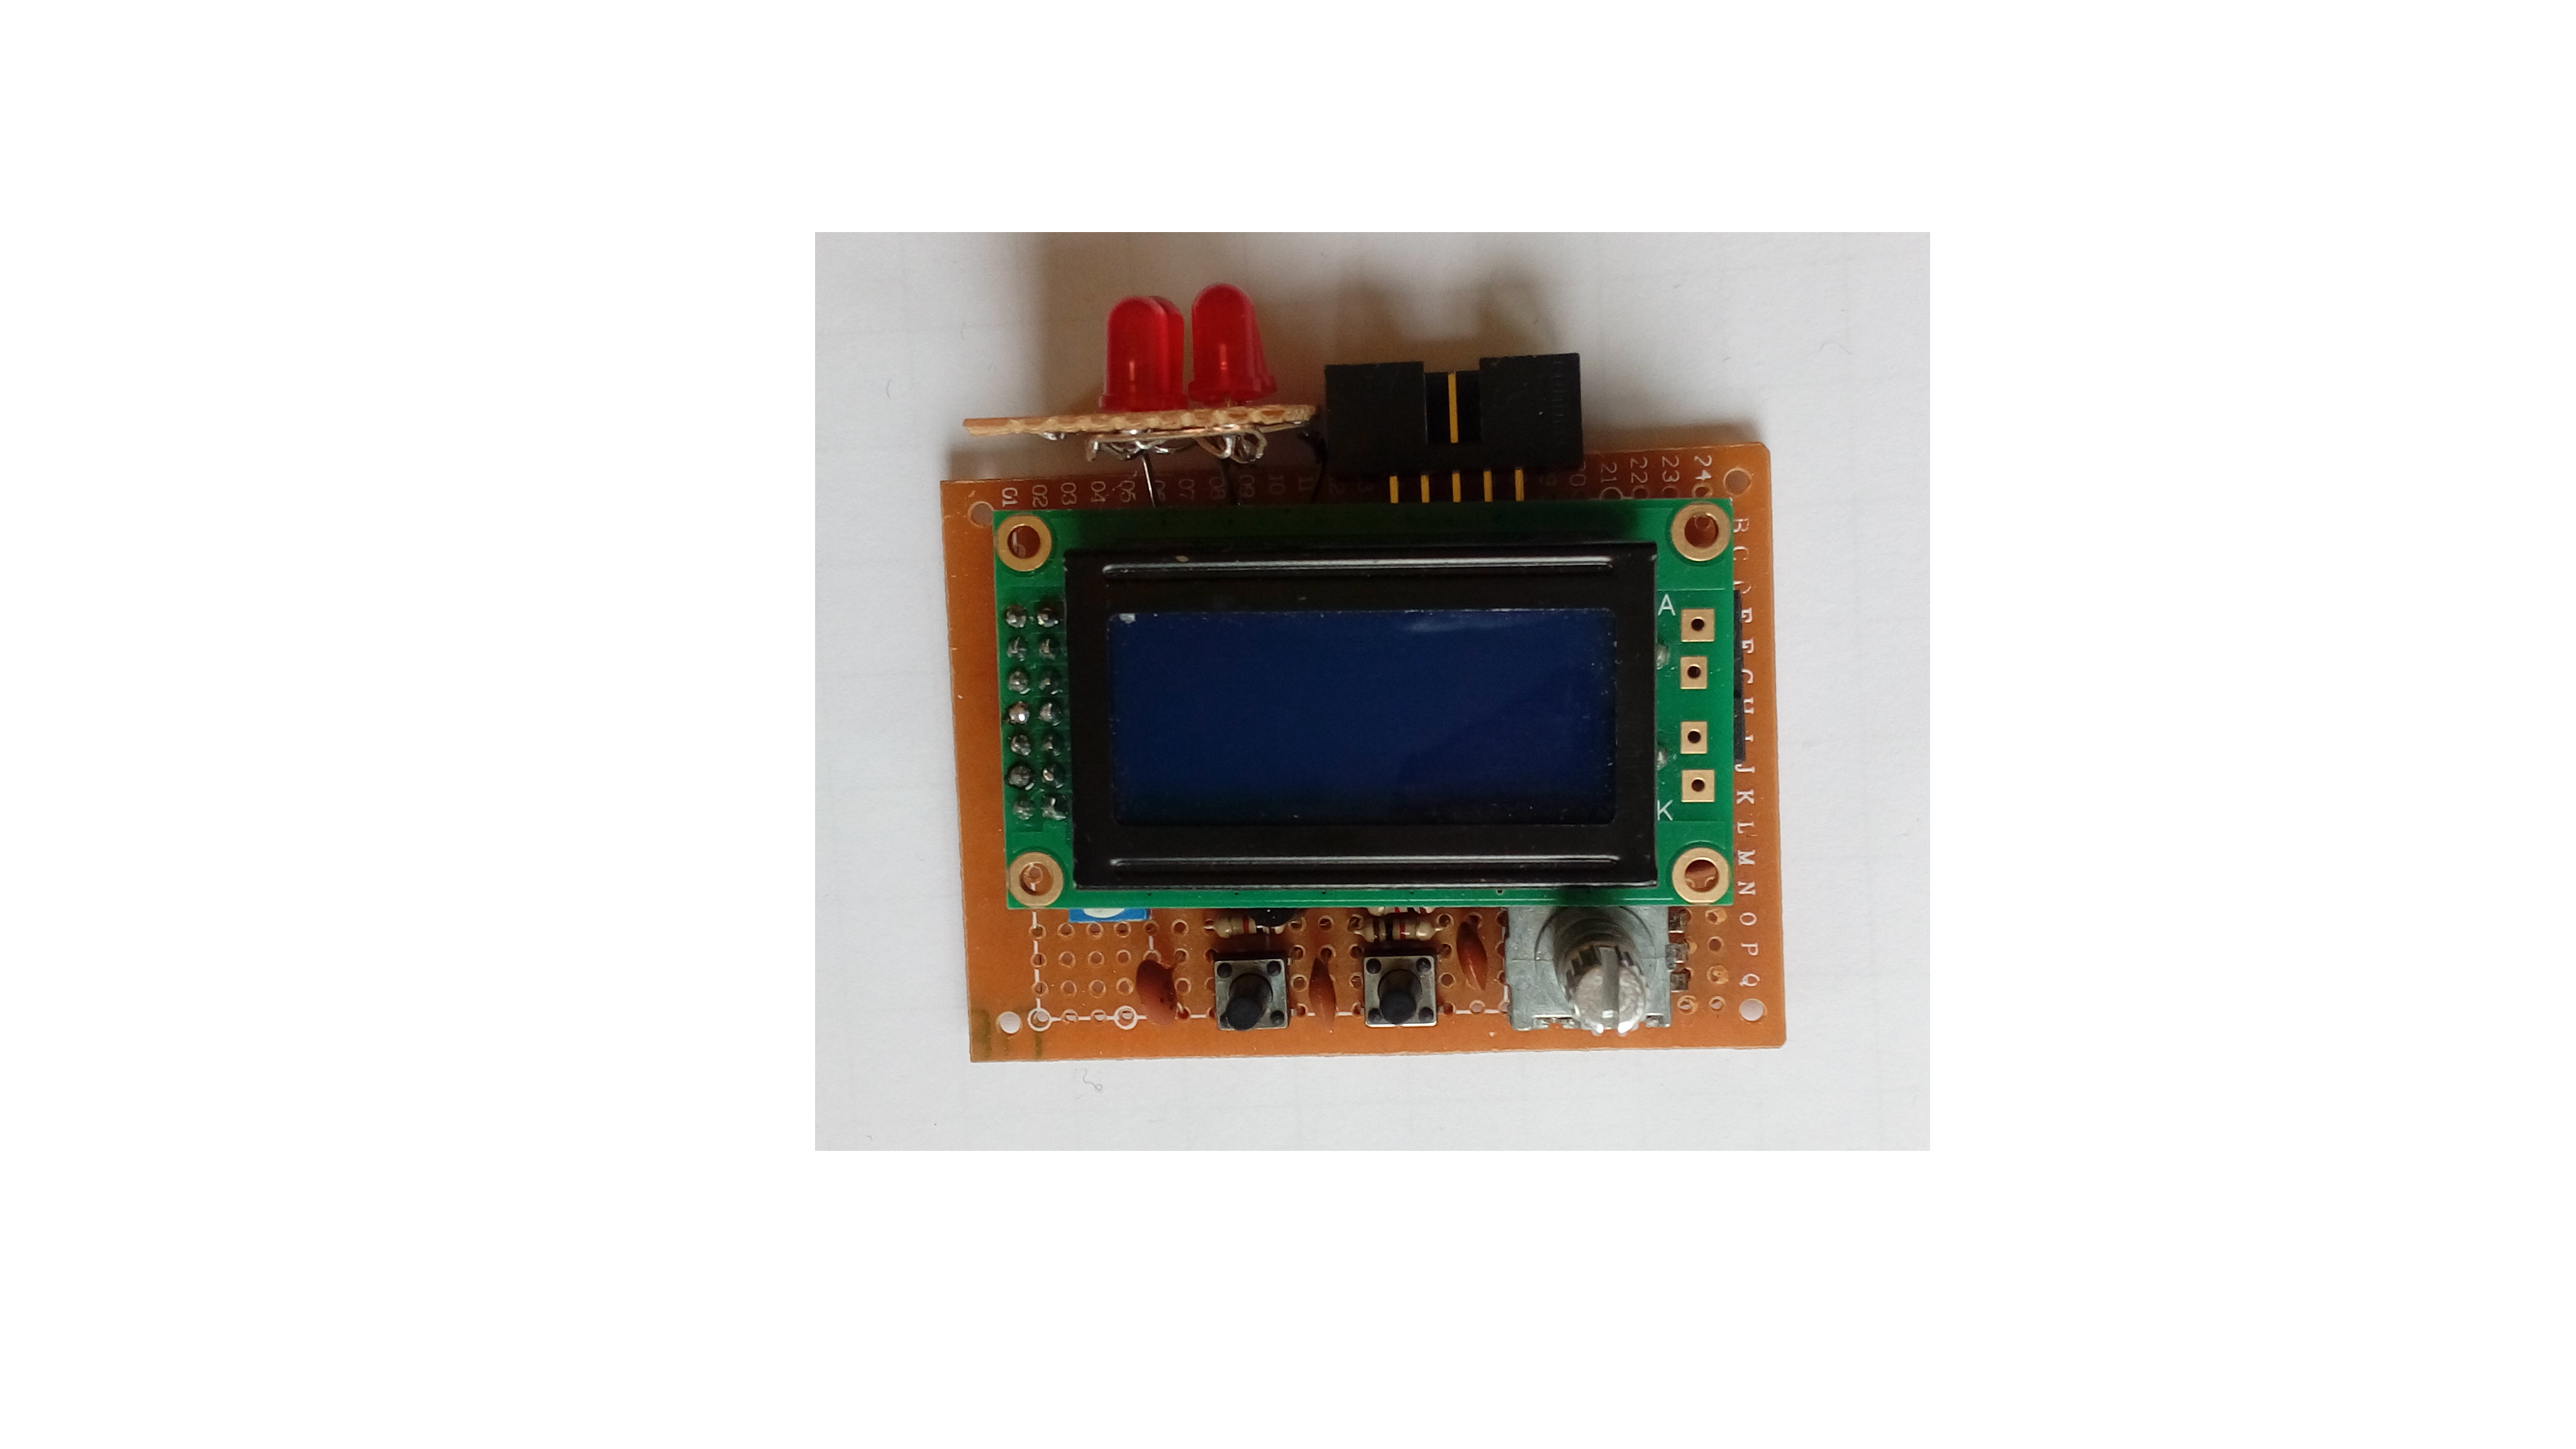
\includegraphics[width=\textwidth]{img/morse_main_view.png}
	%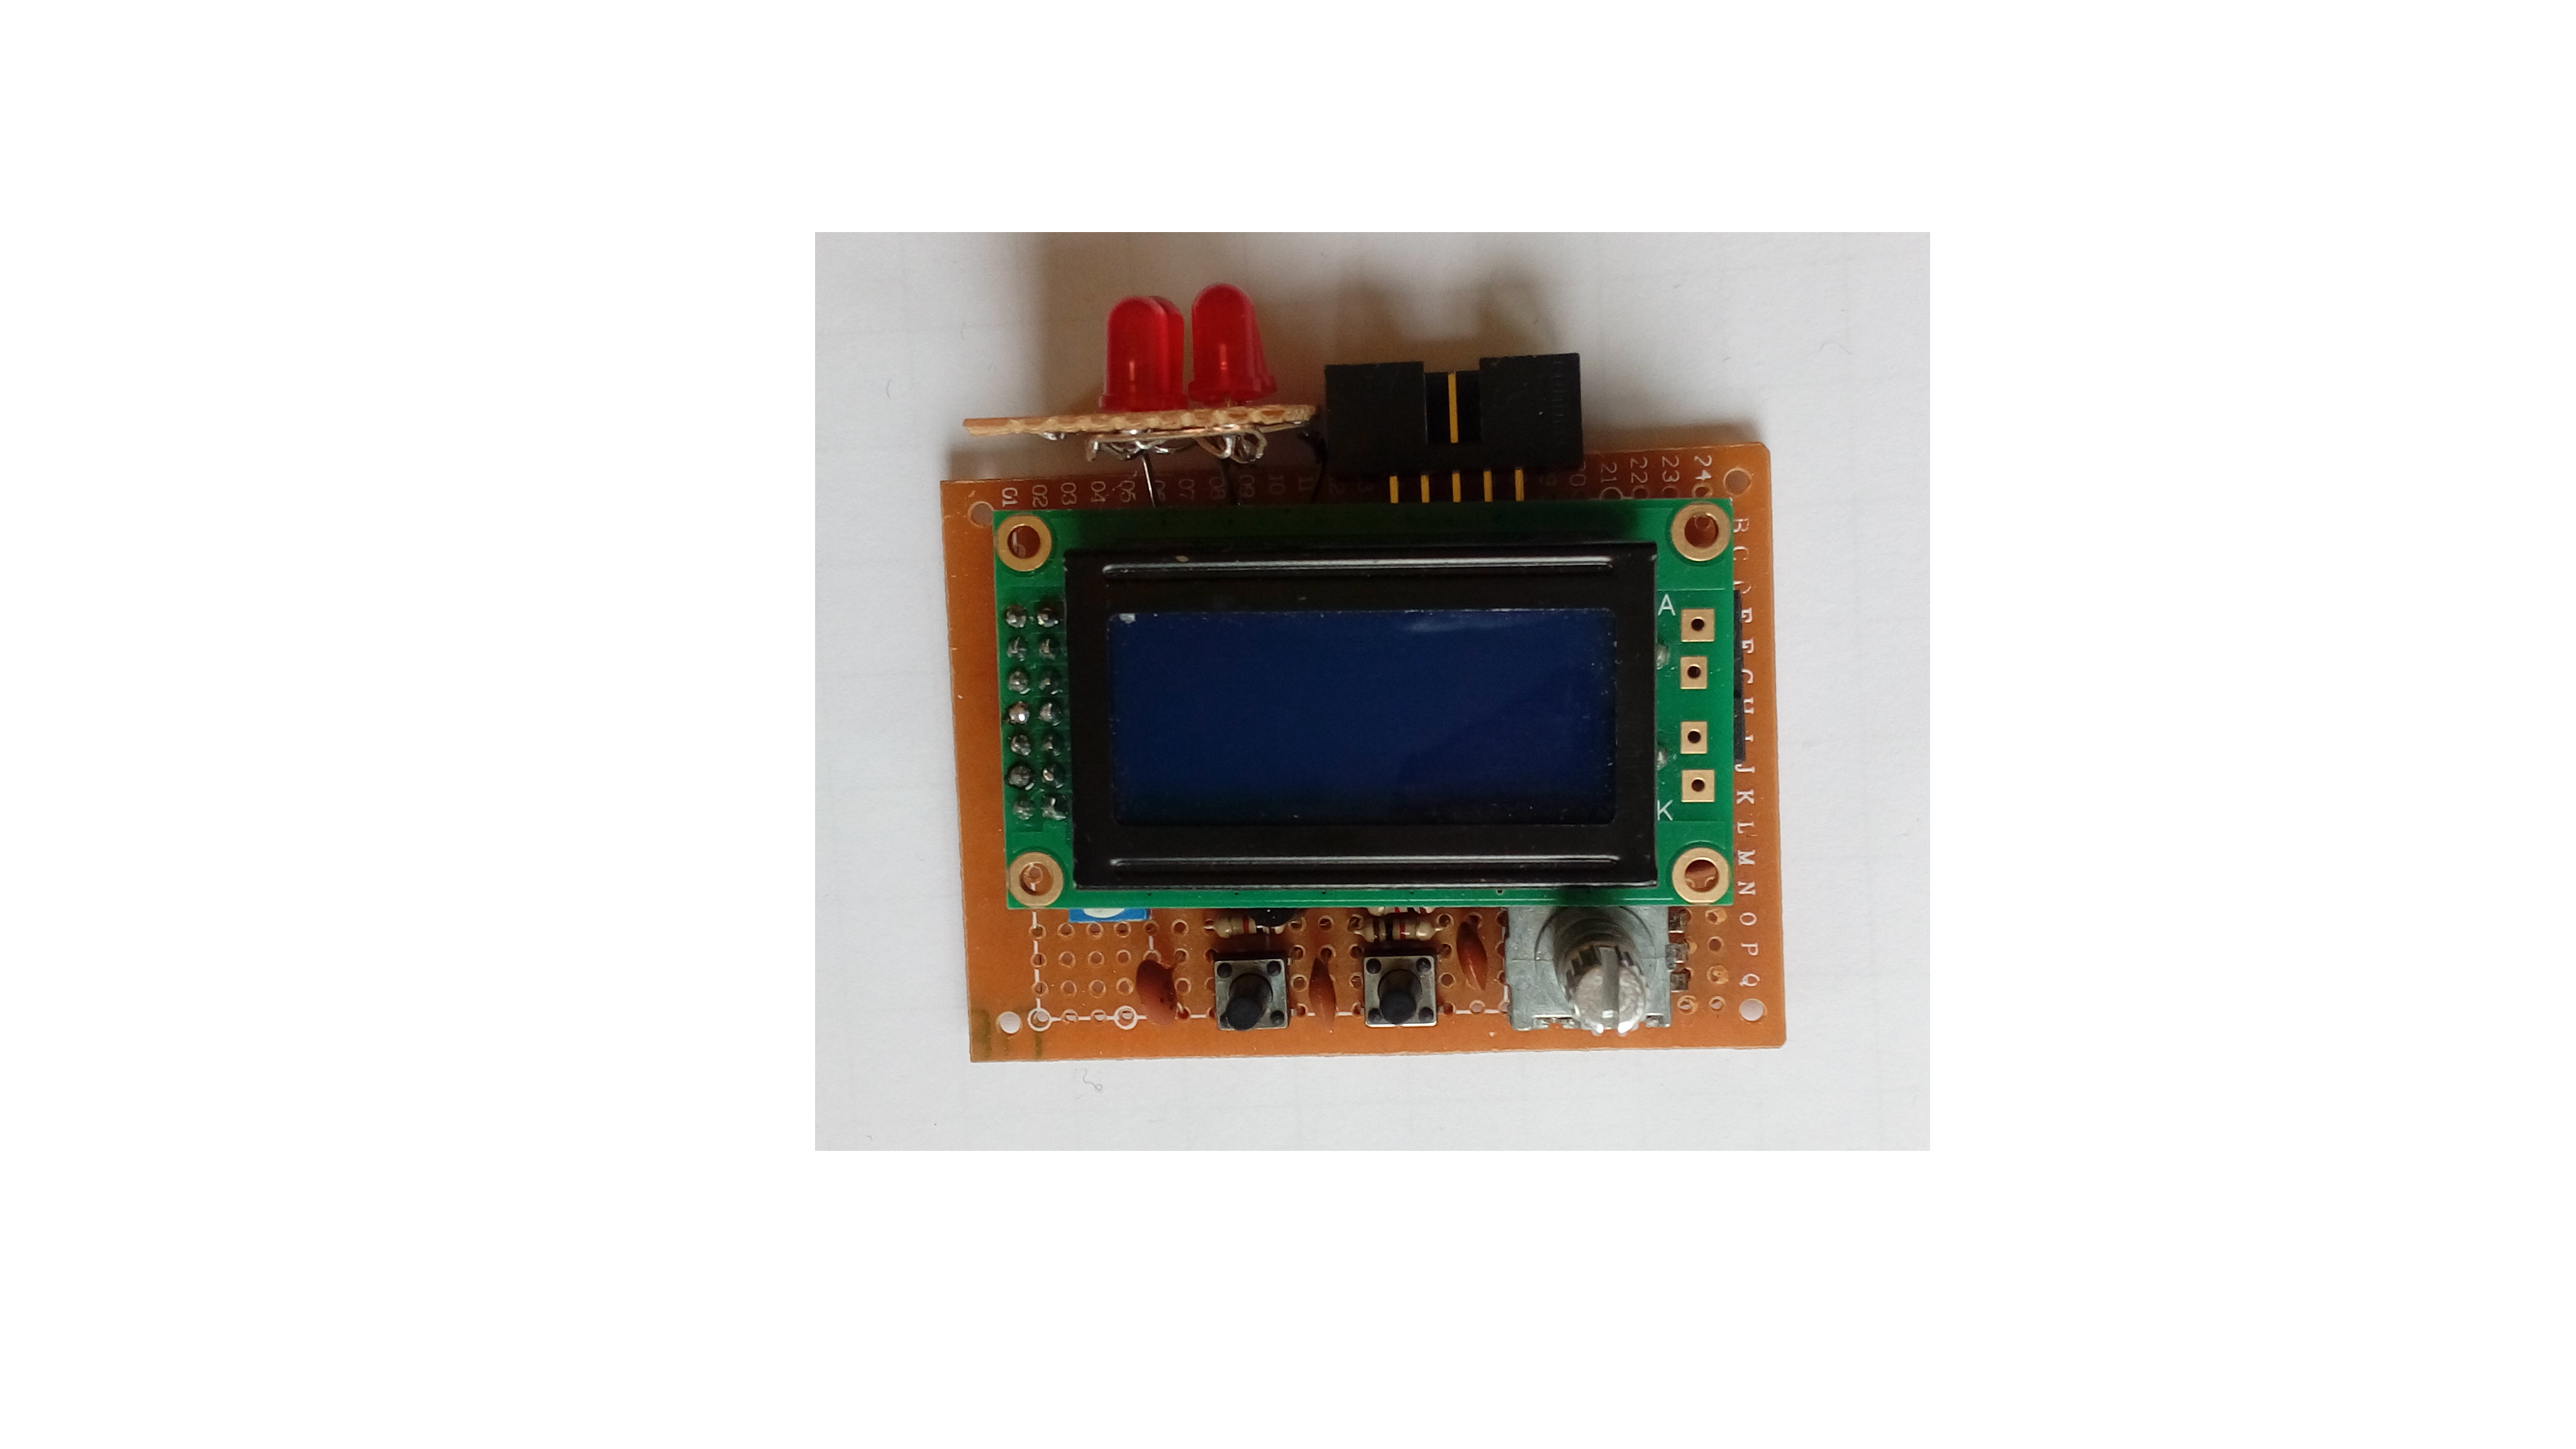
\includegraphics[scale=0.5]{img/morse_main_view.png}
	\caption{Podpis pod obrazkiem}
	\label{fig:zdjecie1}
\end{figure}

\subsection{PROBLEM - Orientacja pozioma}
%\begin{sidewaysfigure}[h!]
%	\centering
%	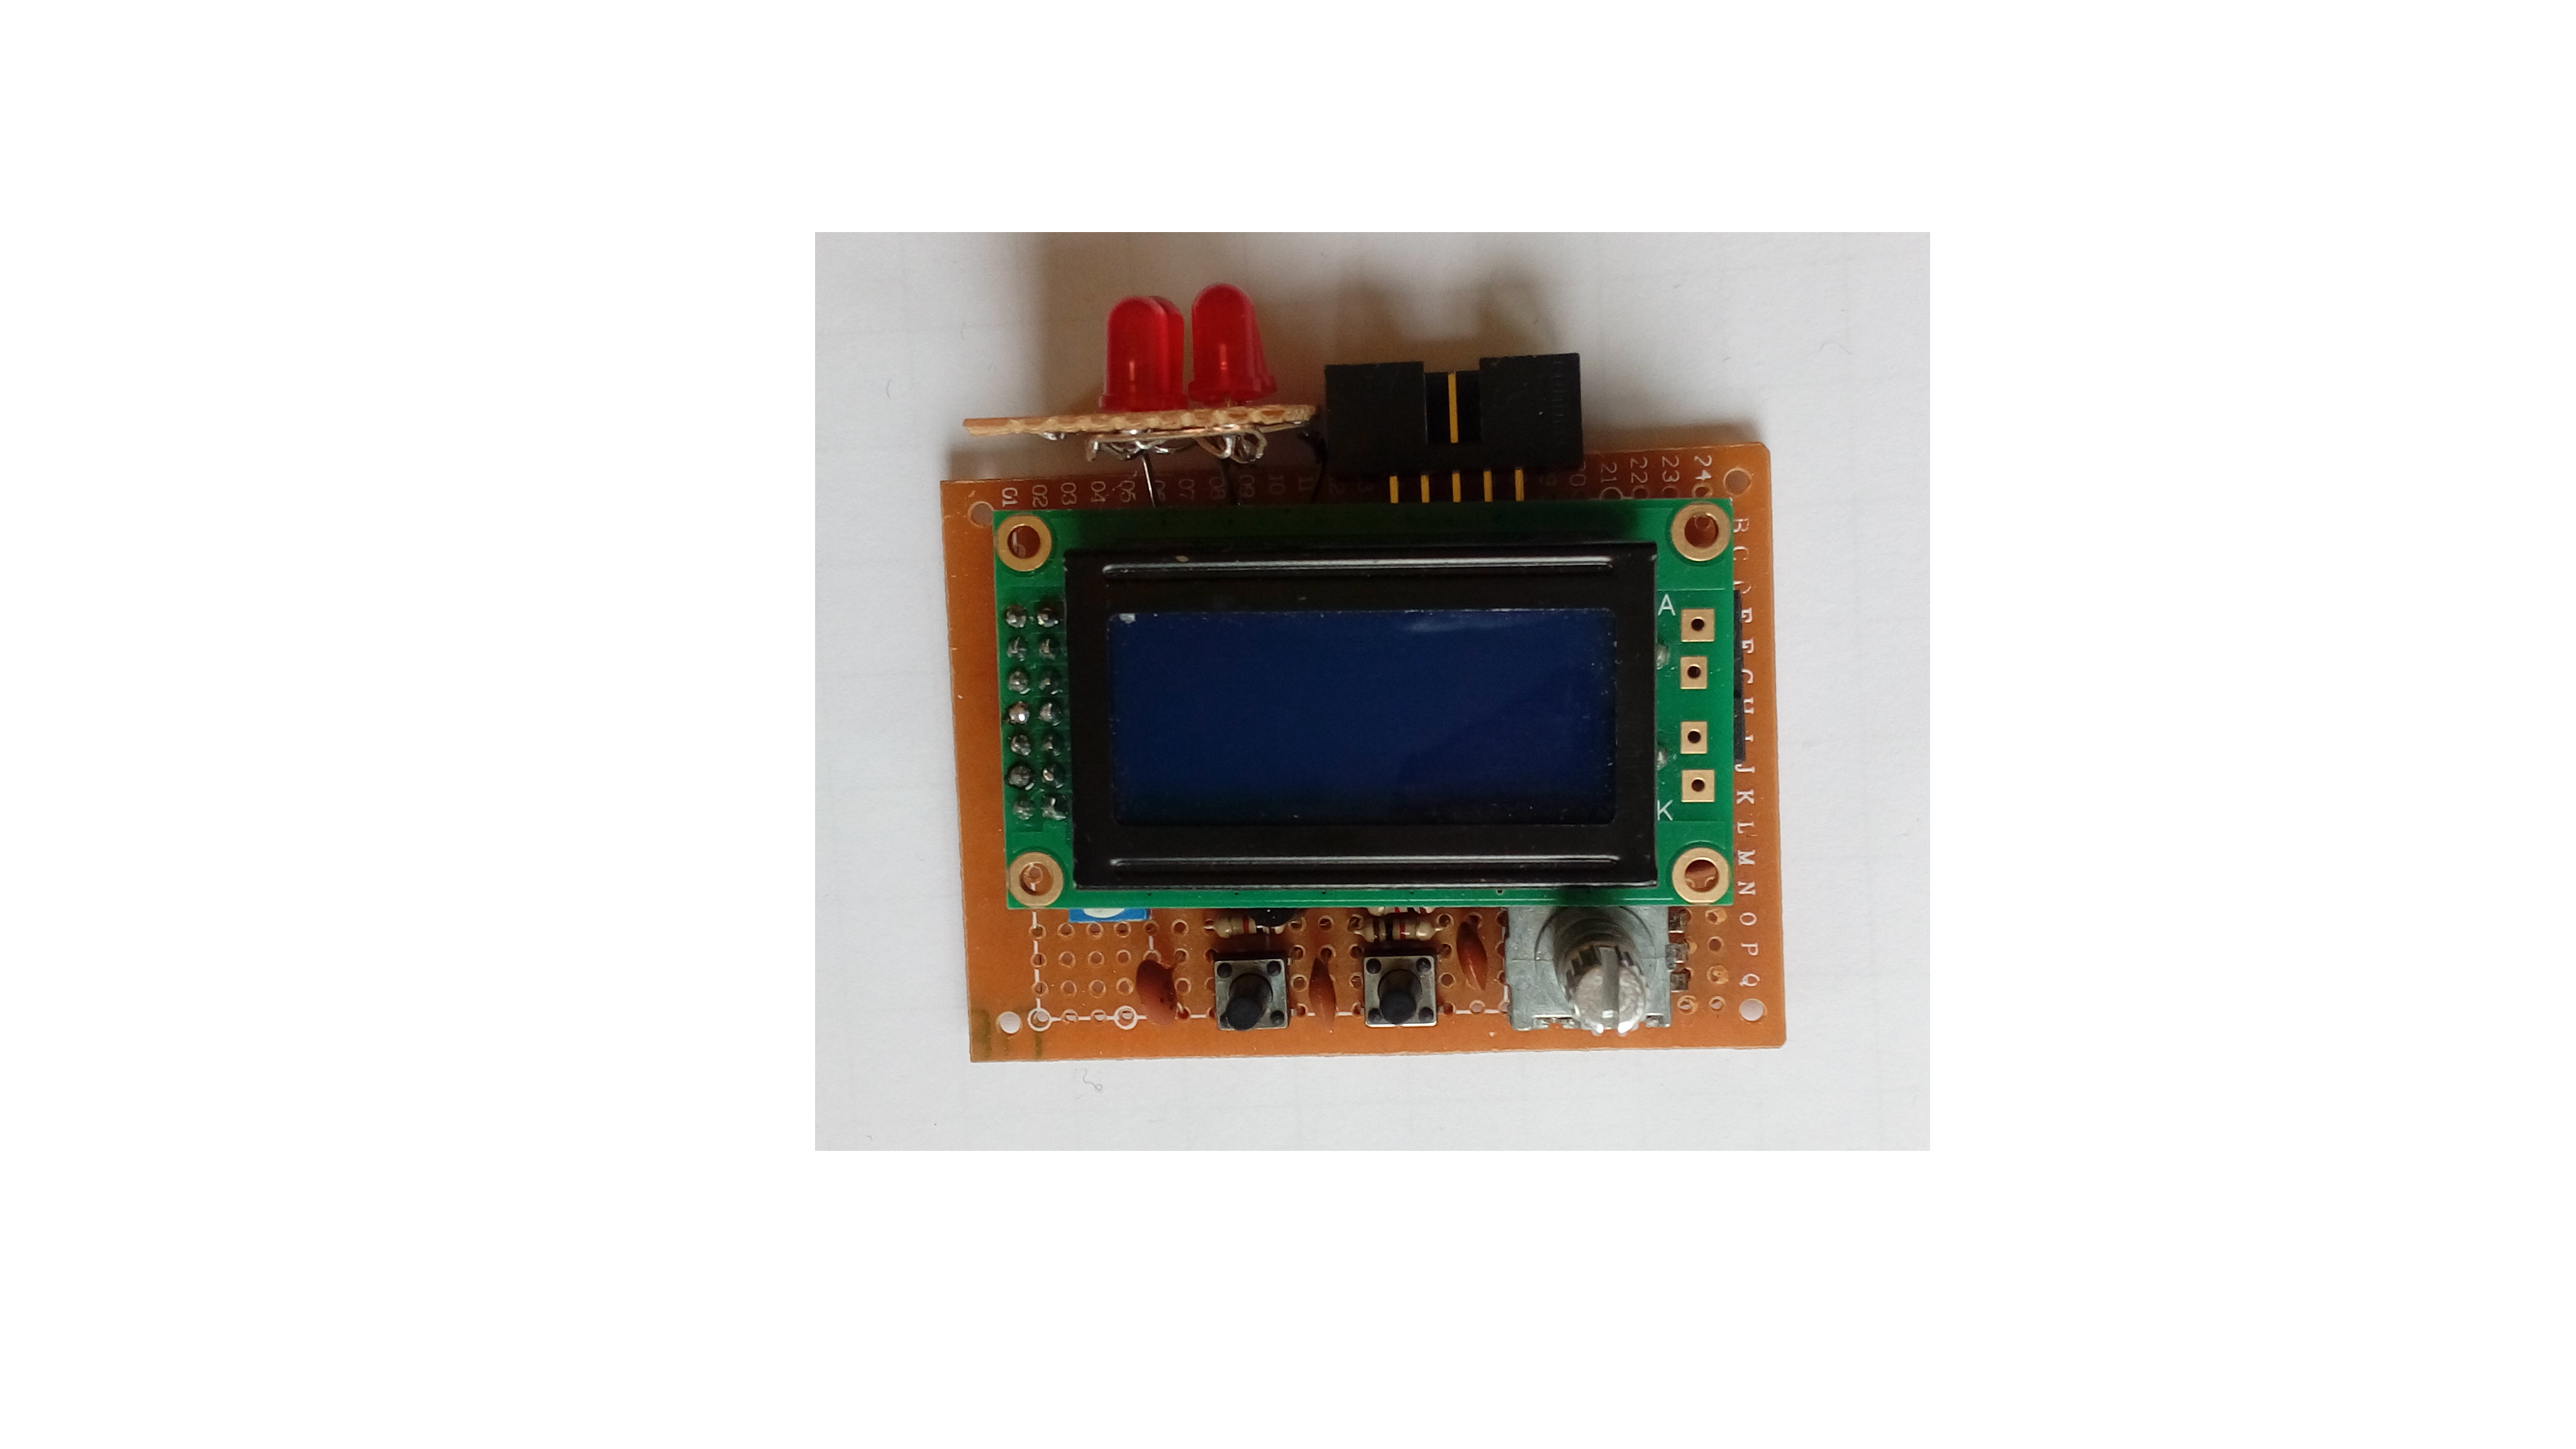
\includegraphics[width=\textwidth]{img/morse_main_view.png}
%	\caption{podpis pod obrazkiem odwróconym}
%	\label{fig:schemat1}
%\end{sidewaysfigure}

\subsection{Zestawienie obrazów}
\begin{figure}[H]
\centering

    \subfloat[podpis jeden]{%
      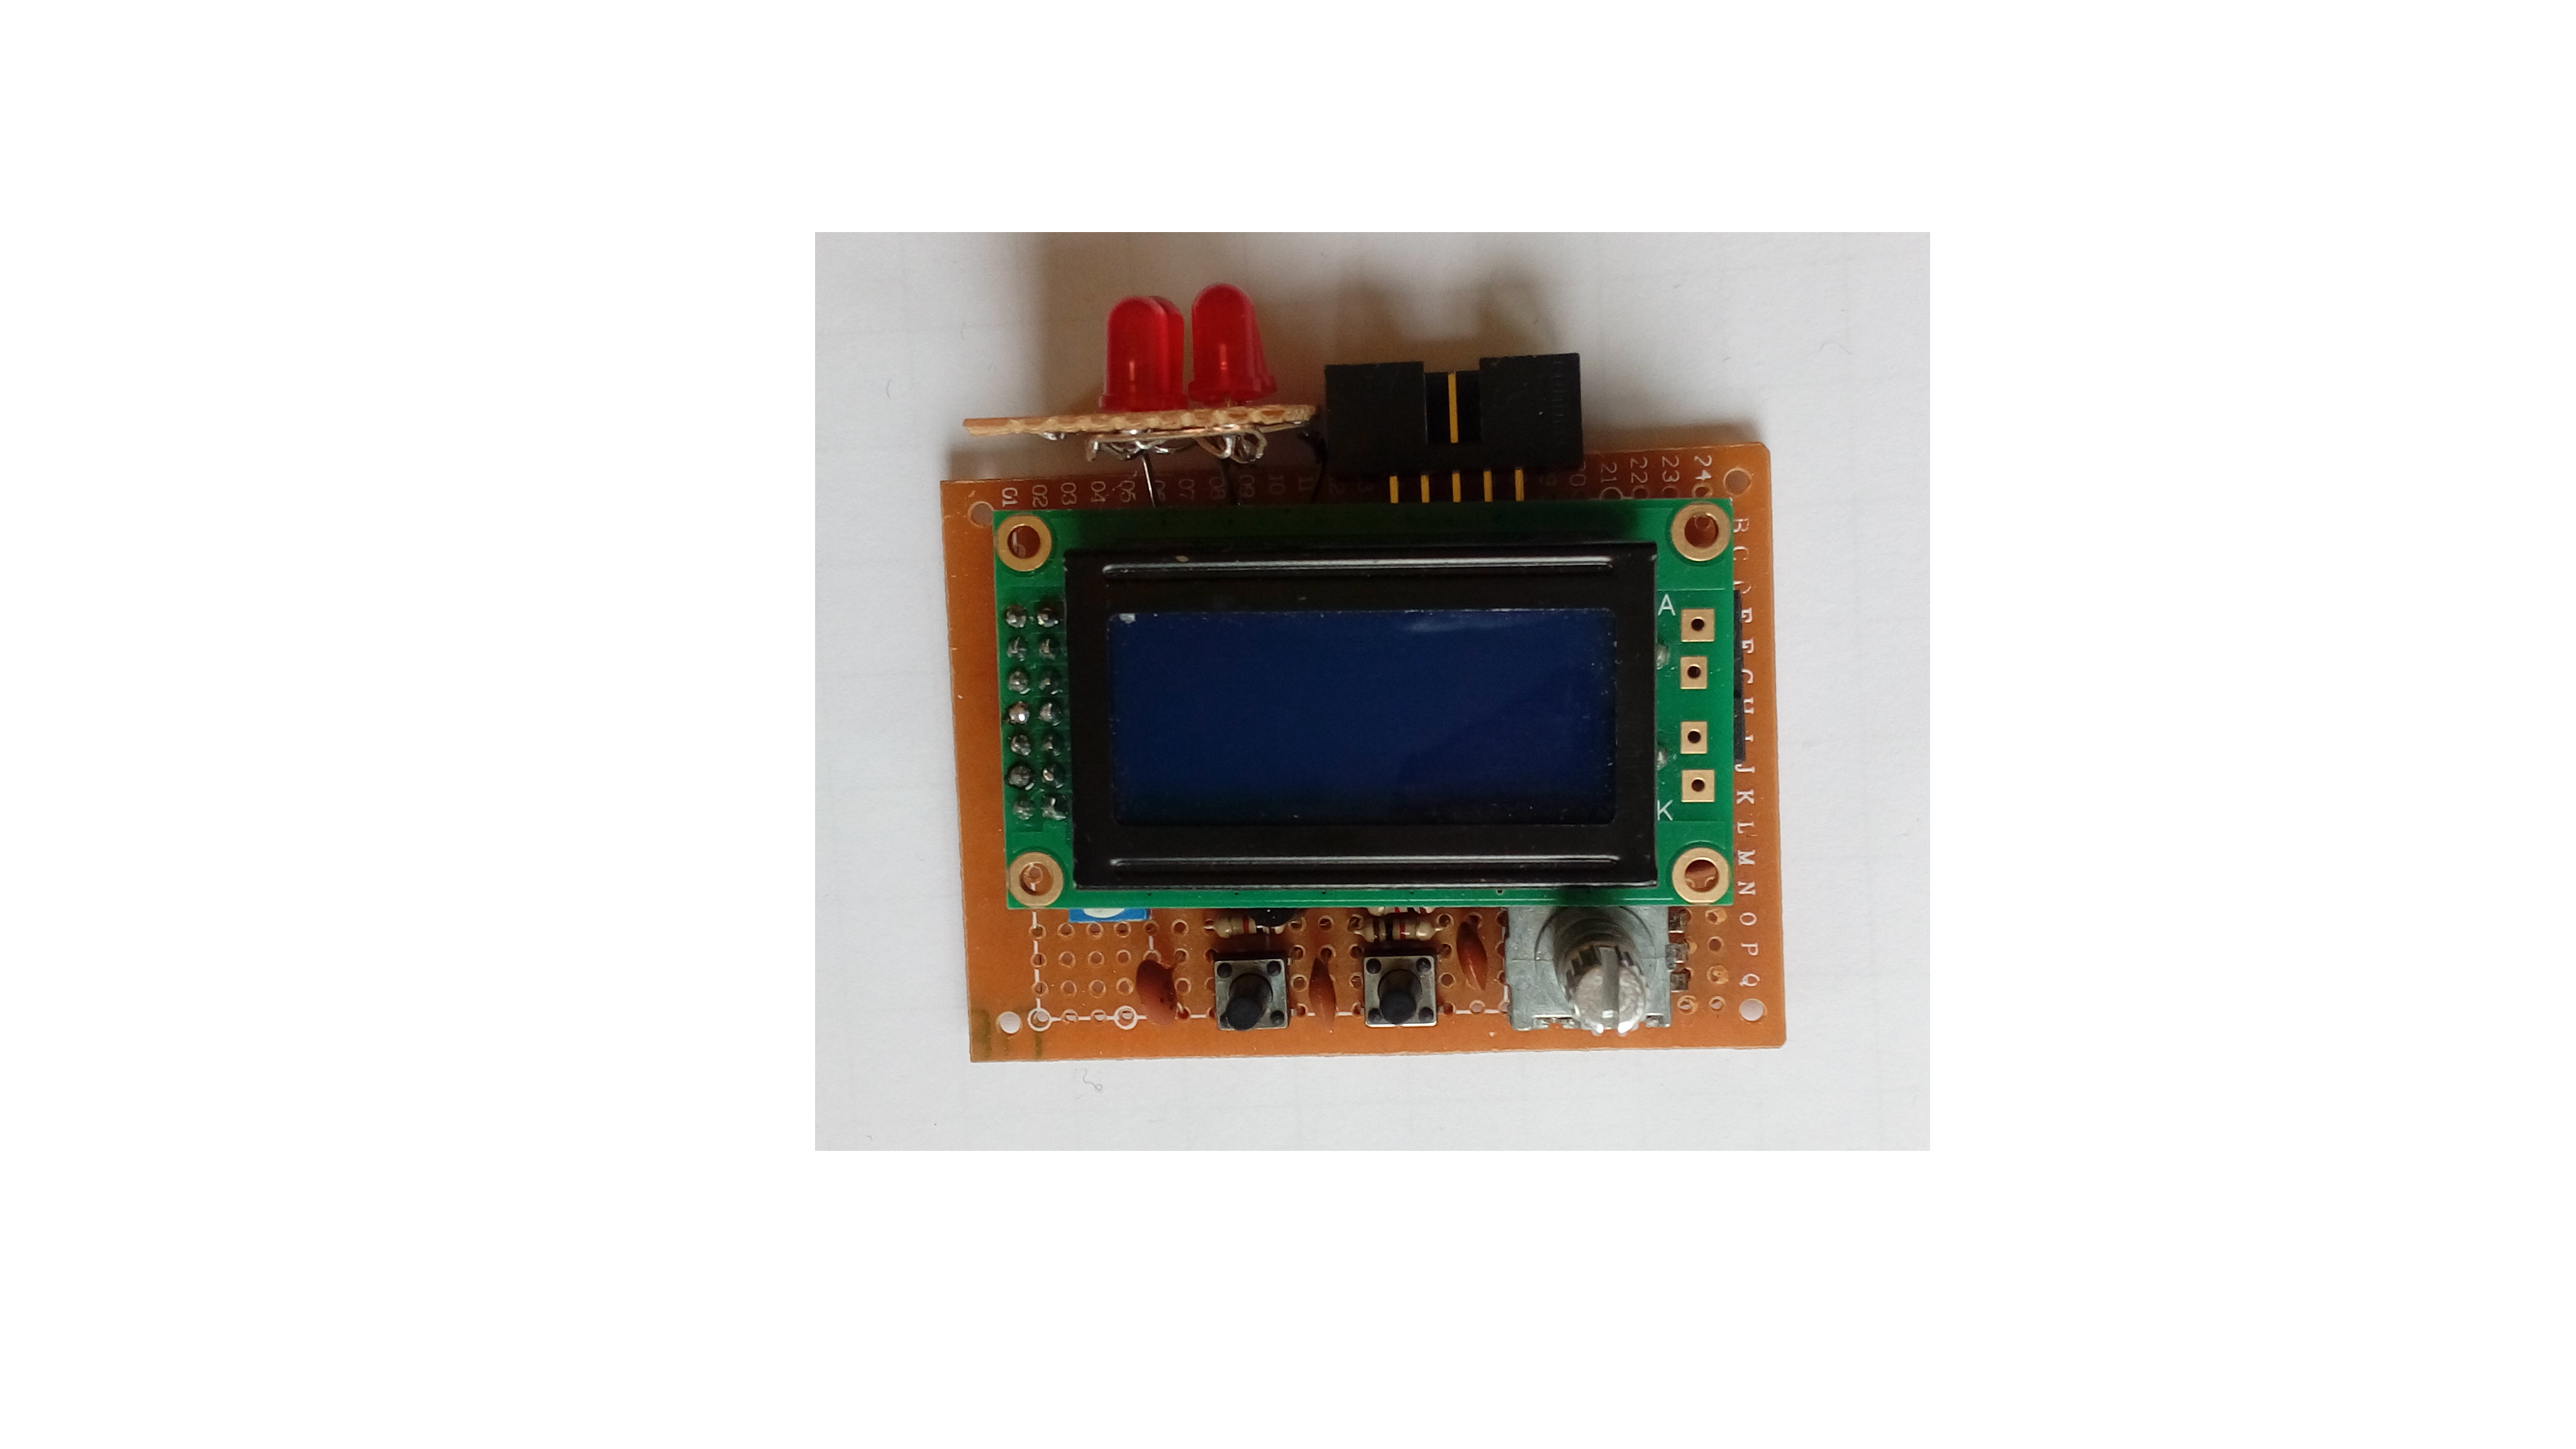
\includegraphics[width=0.4\textwidth]{img/morse_main_view.png}
    } %Miedzy tymi obrazkami nie ma przerwy, wiec beda zestawione poziomo
    \hspace{0.4cm}
    \subfloat[podpis dwa]{%
      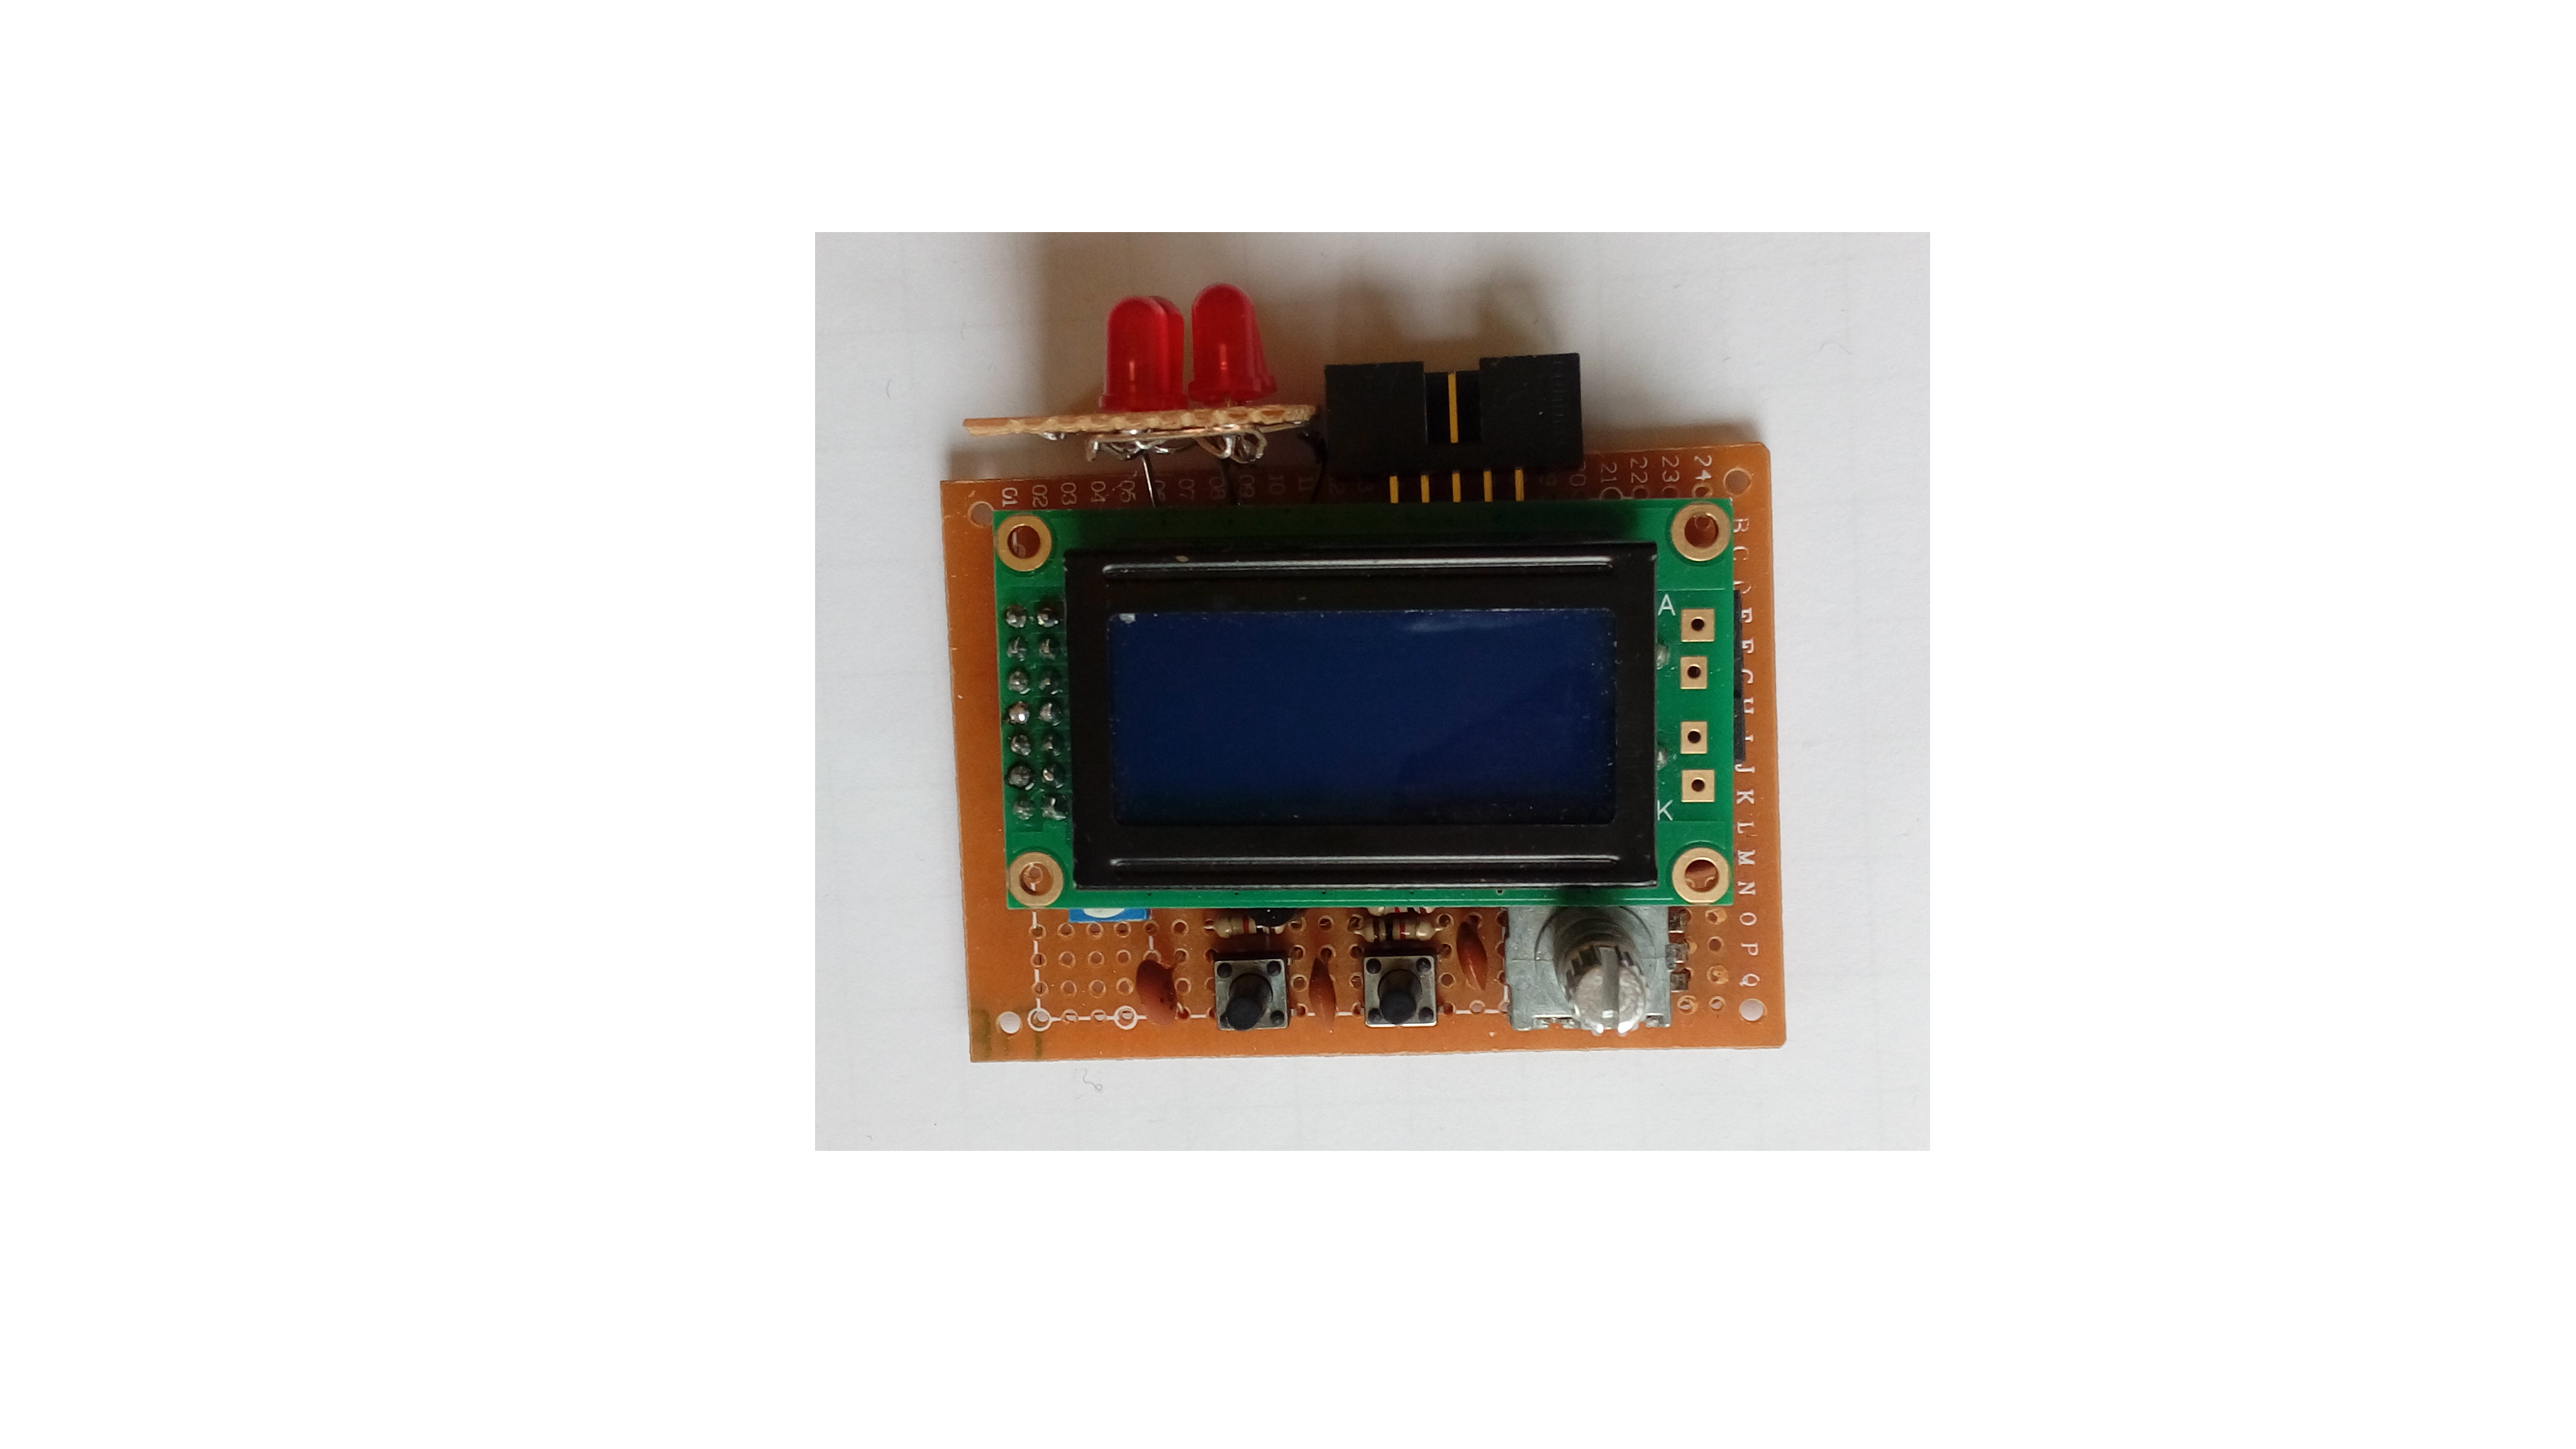
\includegraphics[width=0.4\textwidth]{img/morse_main_view.png}
    }%Ponizej jest przerwa, wiec nastapi przejscie do nowej linii

	\subfloat[podpis trzy]{%
      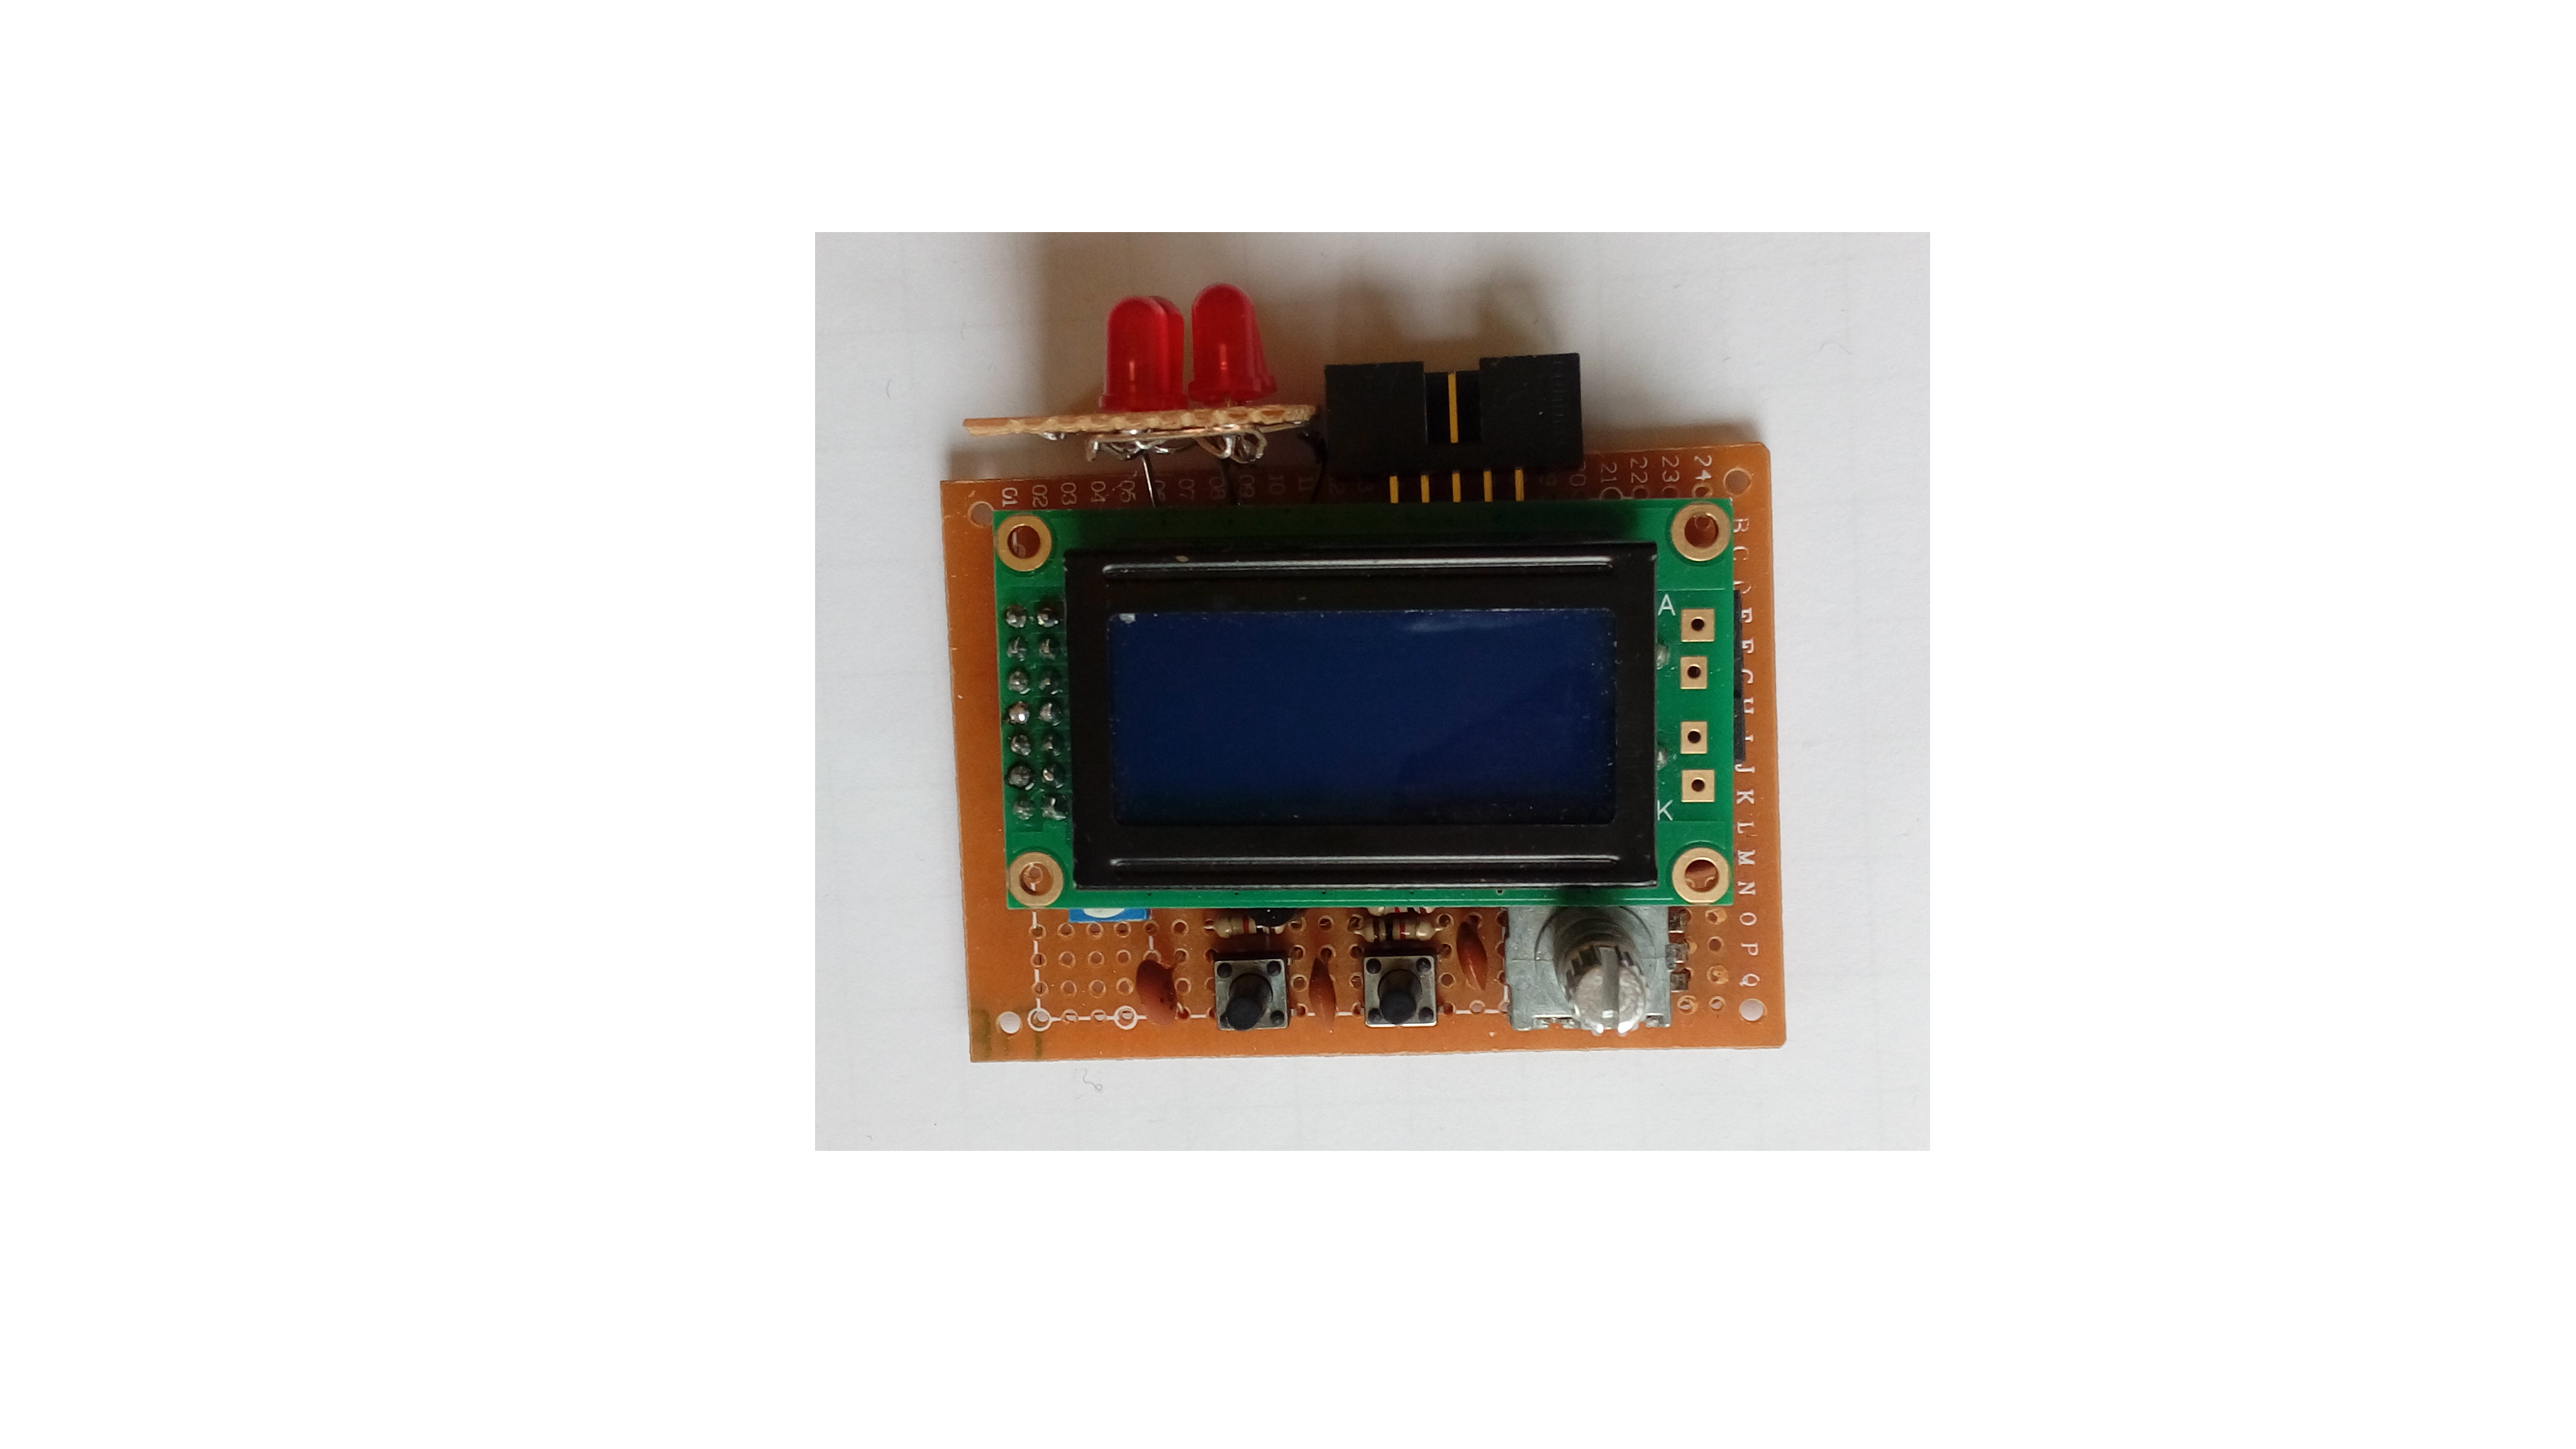
\includegraphics[width=0.9\textwidth]{img/morse_main_view.png}
    }
  \end{figure}%

\section{Wyrównanie tekstu}

\begin{flushright}
Blok tekstu wyrównany do prawej krawędzi dokumentu
\end{flushright}

\begin{center}
Blok tekstu wyrównany do środka dokumentu
\end{center}

\begin{flushleft}
Blok tekstu wyrównany do lewej krawędzi dokumentu
\end{flushleft}

\section{Podział na kolumny}

\begin{multicols}{2}	% liczba kolumn
\lstset{tabsize=1}		% rozmiar wcięcia przed tekstem

Lorem ipsum dolor sit amet, consectetur adipisicing elit, sed do eiusmod tempor incididunt ut labore et dolore magna aliqua. Ut enim ad minim veniam, quis nostrud exercitation ullamco laboris nisi ut aliquip ex ea commodo consequat. Duis aute irure dolor in reprehenderit in voluptate velit esse cillum dolore eu fugiat nulla pariatur. Excepteur sint occaecat cupidatat non proident, sunt in culpa qui officia deserunt mollit anim id est laborum.

\end{multicols}

\section{podział na minipage}

\begin{center}
\begin{minipage}[t]{0.47\textwidth}
	\begin{minipage}[t]{0.3\textwidth}
		\begin{flushright}
			\large{praktykant:\\nr indeksu:\\kierunek:\\wydział:}
		\end{flushright}
	\end{minipage} 
	%
	\begin{minipage}[t]{0.7\textwidth}
		\begin{flushleft}
			\large{\quad Maciej Mielcarski\\
			\quad 235703\\
			\quad Automatyka i Robotyka\\
			\quad Elektroniki W - 4}
		\end{flushleft}
	\end{minipage} 
\end{minipage} 
\end{center}

\section{Wyświetlanie kodu}
\subsection{zwykły monospace}
\lstset{tabsize=1}
\begin{lstlisting}
int main()
{
cout<<"hello world"<<endl;
return 0;
}
\end{lstlisting}
\subsection{Wyróżnianie słów kluczowych}
\begin{minted}[tabsize=3,obeytabs]{c}
int main()
{
	cout<<"hello world"<<endl;
	return 0;
}
\end{minted}

\section{WIĘCEJ - Wzory matematyczne}

\[  
	 R4 = \frac{0.45V}{I_{max}}=\frac{0.45V}{0.35A}=1.2857~\Omega \approx 10~\Omega
\]

\section{Linki}
\href{https://github.com/MMielcarski}{\large\textbf{https://github.com/MMielcarski}}

\section{Przydatne komendy}
tab\quad tab\quad tab \qquad dwa taby \quad\quad\quad\quad itd... \\
wstawienie znaków \$, \#, \_ \\
wstawienie znaku \textbar \\
wstawienie znaku \textgreater \\ 	
\verb$\\$ - nowa linia \\
\verb$\\~\\$ - dwie nowe linie \\
\verb$\maketitle$ - wstawienie strony tytułowej \\
\verb$\newpage$ - przejście do nowej strony \\
\verb$\pagenumbering{gobble}$ - wyłączenie numeracji stron \\
\verb$\pagenumbering{arabic}$ - przywrócenie numeracji stron \\
\verb$\input{title/plik.tex}$ - wstawienie pliku .tex \\
%\href{http://miktex.org} - wstawienie linku

\end{document}